\documentclass[1p]{elsarticle_modified}
%\bibliographystyle{elsarticle-num}

%\usepackage[colorlinks]{hyperref}
%\usepackage{abbrmath_seonhwa} %\Abb, \Ascr, \Acal ,\Abf, \Afrak
\usepackage{amsfonts}
\usepackage{amssymb}
\usepackage{amsmath}
\usepackage{amsthm}
\usepackage{scalefnt}
\usepackage{amsbsy}
\usepackage{kotex}
\usepackage{caption}
\usepackage{subfig}
\usepackage{color}
\usepackage{graphicx}
\usepackage{xcolor} %% white, black, red, green, blue, cyan, magenta, yellow
\usepackage{float}
\usepackage{setspace}
\usepackage{hyperref}

\usepackage{tikz}
\usetikzlibrary{arrows}

\usepackage{multirow}
\usepackage{array} % fixed length table
\usepackage{hhline}

%%%%%%%%%%%%%%%%%%%%%
\makeatletter
\renewcommand*\env@matrix[1][\arraystretch]{%
	\edef\arraystretch{#1}%
	\hskip -\arraycolsep
	\let\@ifnextchar\new@ifnextchar
	\array{*\c@MaxMatrixCols c}}
\makeatother %https://tex.stackexchange.com/questions/14071/how-can-i-increase-the-line-spacing-in-a-matrix
%%%%%%%%%%%%%%%

\usepackage[normalem]{ulem}

\newcommand{\msout}[1]{\ifmmode\text{\sout{\ensuremath{#1}}}\else\sout{#1}\fi}
%SOURCE: \msout is \stkout macro in https://tex.stackexchange.com/questions/20609/strikeout-in-math-mode

\newcommand{\cancel}[1]{
	\ifmmode
	{\color{red}\msout{#1}}
	\else
	{\color{red}\sout{#1}}
	\fi
}

\newcommand{\add}[1]{
	{\color{blue}\uwave{#1}}
}

\newcommand{\replace}[2]{
	\ifmmode
	{\color{red}\msout{#1}}{\color{blue}\uwave{#2}}
	\else
	{\color{red}\sout{#1}}{\color{blue}\uwave{#2}}
	\fi
}

\newcommand{\Sol}{\mathcal{S}} %segment
\newcommand{\D}{D} %diagram
\newcommand{\A}{\mathcal{A}} %arc


%%%%%%%%%%%%%%%%%%%%%%%%%%%%%5 test

\def\sl{\operatorname{\textup{SL}}(2,\Cbb)}
\def\psl{\operatorname{\textup{PSL}}(2,\Cbb)}
\def\quan{\mkern 1mu \triangleright \mkern 1mu}

\theoremstyle{definition}
\newtheorem{thm}{Theorem}[section]
\newtheorem{prop}[thm]{Proposition}
\newtheorem{lem}[thm]{Lemma}
\newtheorem{ques}[thm]{Question}
\newtheorem{cor}[thm]{Corollary}
\newtheorem{defn}[thm]{Definition}
\newtheorem{exam}[thm]{Example}
\newtheorem{rmk}[thm]{Remark}
\newtheorem{alg}[thm]{Algorithm}

\newcommand{\I}{\sqrt{-1}}
\begin{document}

%\begin{frontmatter}
%
%\title{Boundary parabolic representations of knots up to 8 crossings}
%
%%% Group authors per affiliation:
%\author{Yunhi Cho} 
%\address{Department of Mathematics, University of Seoul, Seoul, Korea}
%\ead{yhcho@uos.ac.kr}
%
%
%\author{Seonhwa Kim} %\fnref{s_kim}}
%\address{Center for Geometry and Physics, Institute for Basic Science, Pohang, 37673, Korea}
%\ead{ryeona17@ibs.re.kr}
%
%\author{Hyuk Kim}
%\address{Department of Mathematical Sciences, Seoul National University, Seoul 08826, Korea}
%\ead{hyukkim@snu.ac.kr}
%
%\author{Seokbeom Yoon}
%\address{Department of Mathematical Sciences, Seoul National University, Seoul, 08826,  Korea}
%\ead{sbyoon15@snu.ac.kr}
%
%\begin{abstract}
%We find all boundary parabolic representation of knots up to 8 crossings.
%
%\end{abstract}
%\begin{keyword}
%    \MSC[2010] 57M25 
%\end{keyword}
%
%\end{frontmatter}

%\linenumbers
%\tableofcontents
%
\newcommand\colored[1]{\textcolor{white}{\rule[-0.35ex]{0.8em}{1.4ex}}\kern-0.8em\color{red} #1}%
%\newcommand\colored[1]{\textcolor{white}{ #1}\kern-2.17ex	\textcolor{white}{ #1}\kern-1.81ex	\textcolor{white}{ #1}\kern-2.15ex\color{red}#1	}

{\Large $\underline{11n_{67}~(K11n_{67})}$}

\setlength{\tabcolsep}{10pt}
\renewcommand{\arraystretch}{1.6}
\vspace{1cm}\begin{tabular}{m{100pt}>{\centering\arraybackslash}m{274pt}}
\multirow{5}{120pt}{
	\centering
	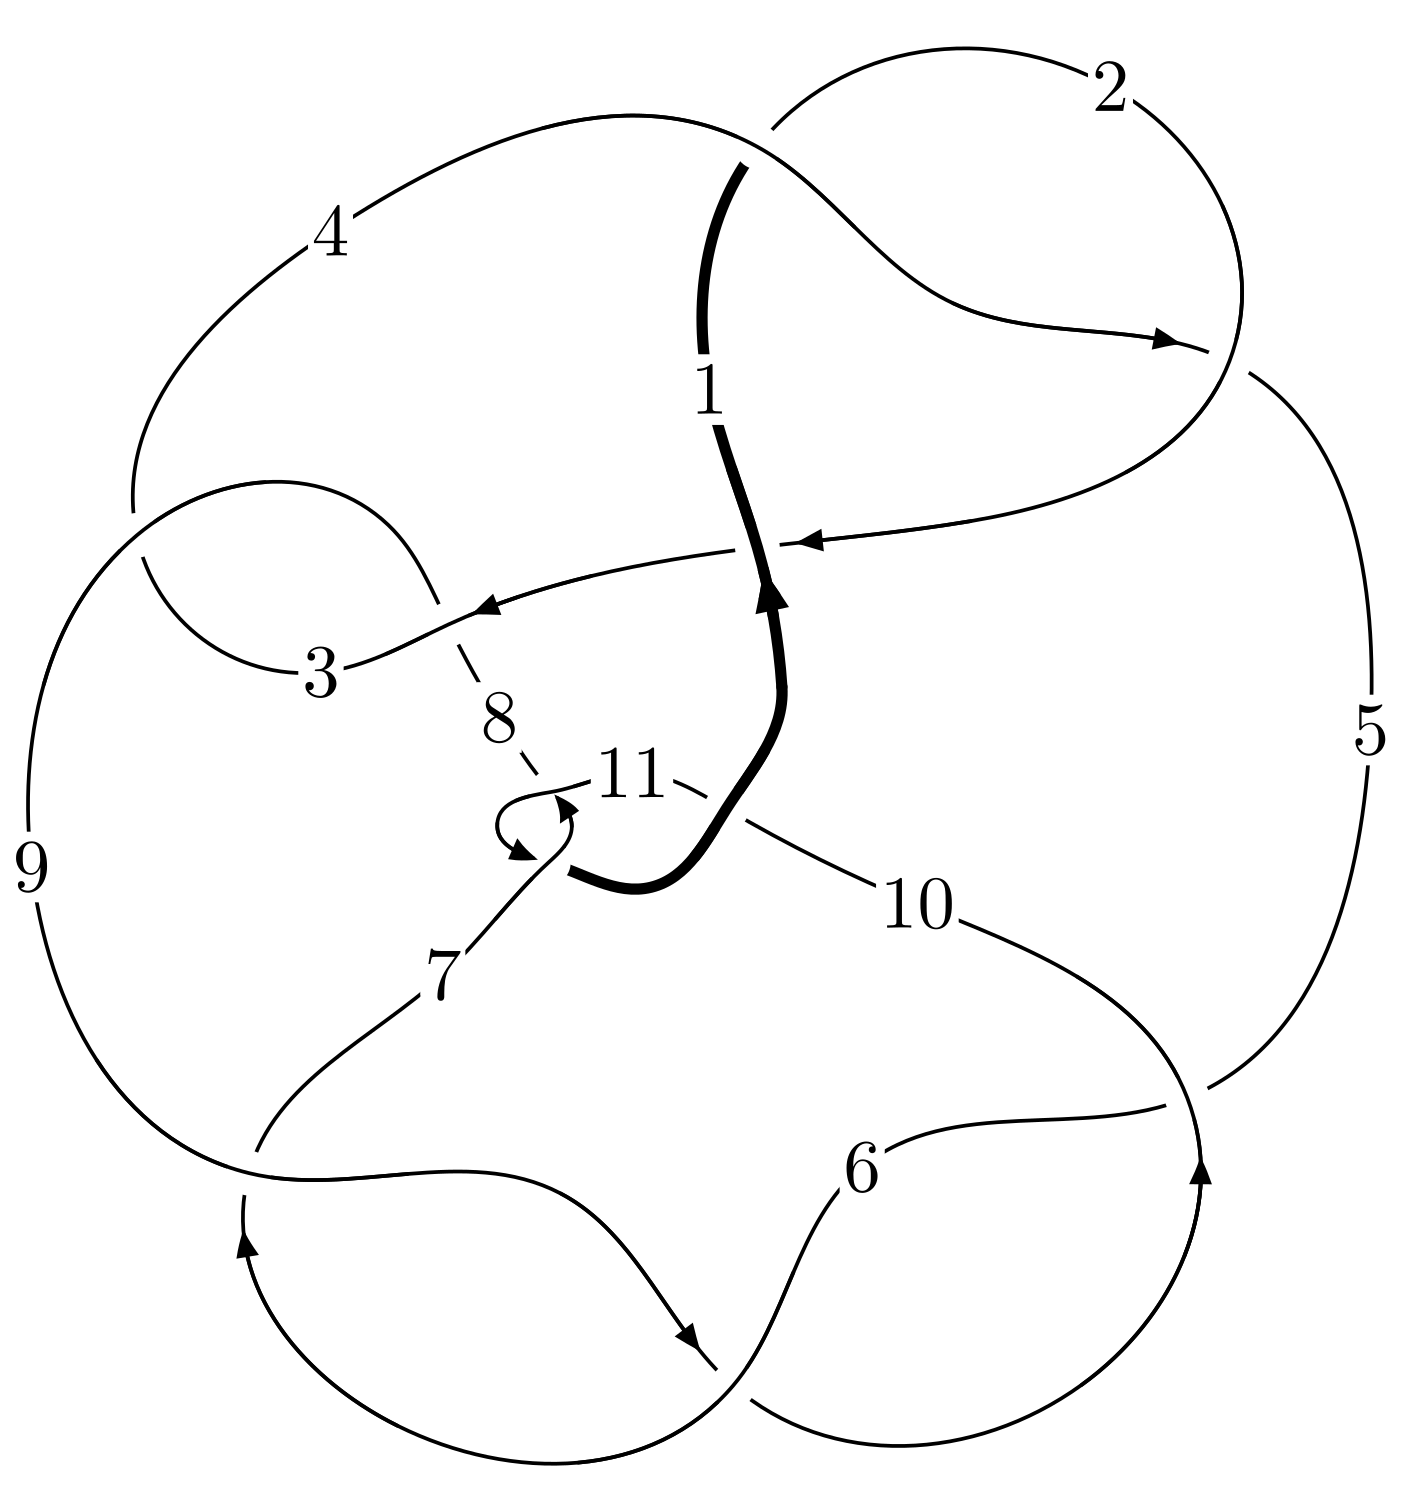
\includegraphics[width=112pt]{../../../GIT/diagram.site/Diagrams/png/683_11n_67.png}\\
\ \ \ A knot diagram\footnotemark}&
\allowdisplaybreaks
\textbf{Linearized knot diagam} \\
\cline{2-2}
 &
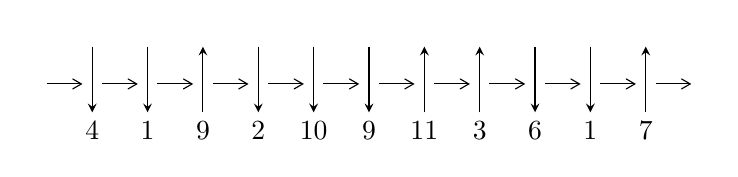
\begin{tikzpicture}[x=20pt, y=17pt]
	% nodes
	\node (C0) at (0, 0) {};
	\node (C1) at (1, 0) {};
	\node (C1U) at (1, +1) {};
	\node (C1D) at (1, -1) {4};

	\node (C2) at (2, 0) {};
	\node (C2U) at (2, +1) {};
	\node (C2D) at (2, -1) {1};

	\node (C3) at (3, 0) {};
	\node (C3U) at (3, +1) {};
	\node (C3D) at (3, -1) {9};

	\node (C4) at (4, 0) {};
	\node (C4U) at (4, +1) {};
	\node (C4D) at (4, -1) {2};

	\node (C5) at (5, 0) {};
	\node (C5U) at (5, +1) {};
	\node (C5D) at (5, -1) {10};

	\node (C6) at (6, 0) {};
	\node (C6U) at (6, +1) {};
	\node (C6D) at (6, -1) {9};

	\node (C7) at (7, 0) {};
	\node (C7U) at (7, +1) {};
	\node (C7D) at (7, -1) {11};

	\node (C8) at (8, 0) {};
	\node (C8U) at (8, +1) {};
	\node (C8D) at (8, -1) {3};

	\node (C9) at (9, 0) {};
	\node (C9U) at (9, +1) {};
	\node (C9D) at (9, -1) {6};

	\node (C10) at (10, 0) {};
	\node (C10U) at (10, +1) {};
	\node (C10D) at (10, -1) {1};

	\node (C11) at (11, 0) {};
	\node (C11U) at (11, +1) {};
	\node (C11D) at (11, -1) {7};
	\node (C12) at (12, 0) {};

	% arrows
	\draw[->,>={angle 60}]
	(C0) edge (C1) (C1) edge (C2) (C2) edge (C3) (C3) edge (C4) (C4) edge (C5) (C5) edge (C6) (C6) edge (C7) (C7) edge (C8) (C8) edge (C9) (C9) edge (C10) (C10) edge (C11) (C11) edge (C12) ;	\draw[->,>=stealth]
	(C1U) edge (C1D) (C2U) edge (C2D) (C3D) edge (C3U) (C4U) edge (C4D) (C5U) edge (C5D) (C6U) edge (C6D) (C7D) edge (C7U) (C8D) edge (C8U) (C9U) edge (C9D) (C10U) edge (C10D) (C11D) edge (C11U) ;
	\end{tikzpicture} \\
\hhline{~~} \\& 
\textbf{Solving Sequence} \\ \cline{2-2} 
 &
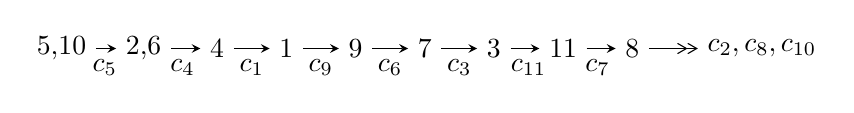
\begin{tikzpicture}[x=25pt, y=7pt]
	% node
	\node (A0) at (-1/8, 0) {5,10};
	\node (A1) at (17/16, 0) {2,6};
	\node (A2) at (17/8, 0) {4};
	\node (A3) at (25/8, 0) {1};
	\node (A4) at (33/8, 0) {9};
	\node (A5) at (41/8, 0) {7};
	\node (A6) at (49/8, 0) {3};
	\node (A7) at (57/8, 0) {11};
	\node (A8) at (65/8, 0) {8};
	\node (C1) at (1/2, -1) {$c_{5}$};
	\node (C2) at (13/8, -1) {$c_{4}$};
	\node (C3) at (21/8, -1) {$c_{1}$};
	\node (C4) at (29/8, -1) {$c_{9}$};
	\node (C5) at (37/8, -1) {$c_{6}$};
	\node (C6) at (45/8, -1) {$c_{3}$};
	\node (C7) at (53/8, -1) {$c_{11}$};
	\node (C8) at (61/8, -1) {$c_{7}$};
	\node (A9) at (10, 0) {$c_{2},c_{8},c_{10}$};

	% edge
	\draw[->,>=stealth]	
	(A0) edge (A1) (A1) edge (A2) (A2) edge (A3) (A3) edge (A4) (A4) edge (A5) (A5) edge (A6) (A6) edge (A7) (A7) edge (A8) ;
	\draw[->>,>={angle 60}]	
	(A8) edge (A9);
\end{tikzpicture} \\ 

\end{tabular} \\

\footnotetext{
The image of knot diagram is generated by the software ``\textbf{Draw programme}" developed by Andrew Bartholomew(\url{http://www.layer8.co.uk/maths/draw/index.htm\#Running-draw}), where we modified some parts for our purpose(\url{https://github.com/CATsTAILs/LinksPainter}).
}\phantom \\ \newline 
\centering \textbf{Ideals for irreducible components\footnotemark of $X_{\text{par}}$} 
 
\begin{align*}
I^u_{1}&=\langle 
-53523809 u^{13}+113678375 u^{12}+\cdots+2227279840 b+1256772587,\\
\phantom{I^u_{1}}&\phantom{= \langle  }-7347336541 u^{13}+13427745311 u^{12}+\cdots+75727514560 a+1617396731,\\
\phantom{I^u_{1}}&\phantom{= \langle  }u^{14}-2 u^{13}+\cdots+24 u+17\rangle \\
I^u_{2}&=\langle 
b+1,\;- u^3+2 u^2+2 a-3 u+5,\;u^4- u^3+3 u^2-2 u+1\rangle \\
I^u_{3}&=\langle 
- a^2 u-2 a^2+4 a u+5 b+3 a-5,\;a^3-3 a^2 u-2 a^2+a u- a+u-2,\;u^2+1\rangle \\
\\
\end{align*}
\raggedright * 3 irreducible components of $\dim_{\mathbb{C}}=0$, with total 24 representations.\\
\footnotetext{All coefficients of polynomials are rational numbers. But the coefficients are sometimes approximated in decimal forms when there is not enough margin.}
\newpage
\renewcommand{\arraystretch}{1}
\centering \section*{I. $I^u_{1}= \langle -5.35\times10^{7} u^{13}+1.14\times10^{8} u^{12}+\cdots+2.23\times10^{9} b+1.26\times10^{9},\;-7.35\times10^{9} u^{13}+1.34\times10^{10} u^{12}+\cdots+7.57\times10^{10} a+1.62\times10^{9},\;u^{14}-2 u^{13}+\cdots+24 u+17 \rangle$}
\flushleft \textbf{(i) Arc colorings}\\
\begin{tabular}{m{7pt} m{180pt} m{7pt} m{180pt} }
\flushright $a_{5}=$&$\begin{pmatrix}1\\0\end{pmatrix}$ \\
\flushright $a_{10}=$&$\begin{pmatrix}0\\u\end{pmatrix}$ \\
\flushright $a_{2}=$&$\begin{pmatrix}0.0970233 u^{13}-0.177317 u^{12}+\cdots+5.72525 u-0.0213581\\0.0240310 u^{13}-0.0510391 u^{12}+\cdots+0.391365 u-0.564263\end{pmatrix}$ \\
\flushright $a_{6}=$&$\begin{pmatrix}1\\u^2\end{pmatrix}$ \\
\flushright $a_{4}=$&$\begin{pmatrix}0.0860286 u^{13}-0.162052 u^{12}+\cdots+4.32173 u+0.0613420\\0.0297616 u^{13}-0.0719847 u^{12}+\cdots+0.0943418 u-0.681013\end{pmatrix}$ \\
\flushright $a_{1}=$&$\begin{pmatrix}0.0390836 u^{13}-0.0710568 u^{12}+\cdots+3.02865 u+0.931294\\0.00745046 u^{13}-0.0211156 u^{12}+\cdots+0.794129 u+0.282743\end{pmatrix}$ \\
\flushright $a_{9}=$&$\begin{pmatrix}u\\u^3+u\end{pmatrix}$ \\
\flushright $a_{7}=$&$\begin{pmatrix}u^2+1\\u^4+2 u^2\end{pmatrix}$ \\
\flushright $a_{3}=$&$\begin{pmatrix}0.0815510 u^{13}-0.158251 u^{12}+\cdots+3.40648 u-0.102474\\0.0311547 u^{13}-0.0816865 u^{12}+\cdots-0.621089 u-0.757212\end{pmatrix}$ \\
\flushright $a_{11}=$&$\begin{pmatrix}0.0118356 u^{13}-0.0182548 u^{12}+\cdots+1.04576 u+0.329948\\-0.00412141 u^{13}+0.0230782 u^{12}+\cdots+1.46293 u+0.190664\end{pmatrix}$ \\
\flushright $a_{8}=$&$\begin{pmatrix}-0.0299569 u^{13}+0.0755900 u^{12}+\cdots+0.453086 u+0.932725\\0.00941903 u^{13}+0.0187909 u^{12}+\cdots+0.243684 u+0.271269\end{pmatrix}$\\ \flushright $a_{8}=$&$\begin{pmatrix}-0.0299569 u^{13}+0.0755900 u^{12}+\cdots+0.453086 u+0.932725\\0.00941903 u^{13}+0.0187909 u^{12}+\cdots+0.243684 u+0.271269\end{pmatrix}$\\&\end{tabular}
\flushleft \textbf{(ii) Obstruction class $= -1$}\\~\\
\flushleft \textbf{(iii) Cusp Shapes $= \frac{159749339}{1781823872} u^{13}-\frac{841106653}{8909119360} u^{12}+\cdots-\frac{20311908351}{8909119360} u-\frac{30534615889}{8909119360}$}\\~\\
\newpage\renewcommand{\arraystretch}{1}
\flushleft \textbf{(iv) u-Polynomials at the component}\newline \\
\begin{tabular}{m{50pt}|m{274pt}}
Crossings & \hspace{64pt}u-Polynomials at each crossing \\
\hline $$\begin{aligned}c_{1},c_{4}\end{aligned}$$&$\begin{aligned}
&u^{14}-7 u^{13}+\cdots+3 u+4
\end{aligned}$\\
\hline $$\begin{aligned}c_{2}\end{aligned}$$&$\begin{aligned}
&u^{14}-3 u^{13}+\cdots-127 u+16
\end{aligned}$\\
\hline $$\begin{aligned}c_{3},c_{8}\end{aligned}$$&$\begin{aligned}
&u^{14}+8 u^{13}+\cdots+80 u+64
\end{aligned}$\\
\hline $$\begin{aligned}c_{5},c_{6},c_{9}\end{aligned}$$&$\begin{aligned}
&u^{14}-2 u^{13}+\cdots+24 u+17
\end{aligned}$\\
\hline $$\begin{aligned}c_{7},c_{11}\end{aligned}$$&$\begin{aligned}
&u^{14}-2 u^{13}+\cdots-12 u+17
\end{aligned}$\\
\hline $$\begin{aligned}c_{10}\end{aligned}$$&$\begin{aligned}
&u^{14}-4 u^{13}+\cdots+2066 u+289
\end{aligned}$\\
\hline
\end{tabular}\\~\\
\newpage\renewcommand{\arraystretch}{1}
\flushleft \textbf{(v) Riley Polynomials at the component}\newline \\
\begin{tabular}{m{50pt}|m{274pt}}
Crossings & \hspace{64pt}Riley Polynomials at each crossing \\
\hline $$\begin{aligned}c_{1},c_{4}\end{aligned}$$&$\begin{aligned}
&y^{14}+3 y^{13}+\cdots+127 y+16
\end{aligned}$\\
\hline $$\begin{aligned}c_{2}\end{aligned}$$&$\begin{aligned}
&y^{14}+47 y^{13}+\cdots+32223 y+256
\end{aligned}$\\
\hline $$\begin{aligned}c_{3},c_{8}\end{aligned}$$&$\begin{aligned}
&y^{14}-42 y^{13}+\cdots+4864 y+4096
\end{aligned}$\\
\hline $$\begin{aligned}c_{5},c_{6},c_{9}\end{aligned}$$&$\begin{aligned}
&y^{14}+28 y^{13}+\cdots+2994 y+289
\end{aligned}$\\
\hline $$\begin{aligned}c_{7},c_{11}\end{aligned}$$&$\begin{aligned}
&y^{14}-4 y^{13}+\cdots+2066 y+289
\end{aligned}$\\
\hline $$\begin{aligned}c_{10}\end{aligned}$$&$\begin{aligned}
&y^{14}+52 y^{13}+\cdots+189758 y+83521
\end{aligned}$\\
\hline
\end{tabular}\\~\\
\newpage\flushleft \textbf{(vi) Complex Volumes and Cusp Shapes}
$$\begin{array}{c|c|c}  
\text{Solutions to }I^u_{1}& \I (\text{vol} + \sqrt{-1}CS) & \text{Cusp shape}\\
 \hline 
\begin{aligned}
u &= -0.739038 + 0.298276 I \\
a &= \phantom{-}0.673213 - 0.315821 I \\
b &= \phantom{-}0.313142 - 0.702457 I\end{aligned}
 & \phantom{-}0.02319 + 2.21939 I & -1.77809 - 3.53992 I \\ \hline\begin{aligned}
u &= -0.739038 - 0.298276 I \\
a &= \phantom{-}0.673213 + 0.315821 I \\
b &= \phantom{-}0.313142 + 0.702457 I\end{aligned}
 & \phantom{-}0.02319 - 2.21939 I & -1.77809 + 3.53992 I \\ \hline\begin{aligned}
u &= -0.267566 + 0.668739 I \\
a &= \phantom{-}0.619498 - 0.223590 I \\
b &= -0.172651 + 0.268532 I\end{aligned}
 & \phantom{-}0.212568 + 1.285480 I & \phantom{-}1.55268 - 6.08941 I \\ \hline\begin{aligned}
u &= -0.267566 - 0.668739 I \\
a &= \phantom{-}0.619498 + 0.223590 I \\
b &= -0.172651 - 0.268532 I\end{aligned}
 & \phantom{-}0.212568 - 1.285480 I & \phantom{-}1.55268 + 6.08941 I \\ \hline\begin{aligned}
u &= \phantom{-}0.01822 + 1.41811 I \\
a &= \phantom{-}0.361569 + 0.414725 I \\
b &= \phantom{-}0.983382 - 0.463084 I\end{aligned}
 & \phantom{-}5.01039 + 4.24504 I & \phantom{-}1.99936 - 6.80413 I \\ \hline\begin{aligned}
u &= \phantom{-}0.01822 - 1.41811 I \\
a &= \phantom{-}0.361569 - 0.414725 I \\
b &= \phantom{-}0.983382 + 0.463084 I\end{aligned}
 & \phantom{-}5.01039 - 4.24504 I & \phantom{-}1.99936 + 6.80413 I \\ \hline\begin{aligned}
u &= \phantom{-}0.120536 + 0.452712 I \\
a &= -3.28623 + 1.15613 I \\
b &= -1.024040 - 0.163148 I\end{aligned}
 & -2.12302 - 0.75753 I & -7.75042 - 3.06748 I \\ \hline\begin{aligned}
u &= \phantom{-}0.120536 - 0.452712 I \\
a &= -3.28623 - 1.15613 I \\
b &= -1.024040 + 0.163148 I\end{aligned}
 & -2.12302 + 0.75753 I & -7.75042 + 3.06748 I \\ \hline\begin{aligned}
u &= \phantom{-}0.60560 + 1.93212 I \\
a &= \phantom{-}0.342835 - 1.047120 I \\
b &= \phantom{-}1.50068 + 1.04479 I\end{aligned}
 & -19.4276 - 10.6503 I & -1.06301 + 4.03963 I \\ \hline\begin{aligned}
u &= \phantom{-}0.60560 - 1.93212 I \\
a &= \phantom{-}0.342835 + 1.047120 I \\
b &= \phantom{-}1.50068 - 1.04479 I\end{aligned}
 & -19.4276 + 10.6503 I & -1.06301 - 4.03963 I\\
 \hline 
 \end{array}$$\newpage$$\begin{array}{c|c|c}  
\text{Solutions to }I^u_{1}& \I (\text{vol} + \sqrt{-1}CS) & \text{Cusp shape}\\
 \hline 
\begin{aligned}
u &= \phantom{-}1.05779 + 1.83805 I \\
a &= \phantom{-}0.405077 - 0.680123 I \\
b &= \phantom{-}0.63249 + 1.72109 I\end{aligned}
 & \phantom{-}9.20003 - 2.06852 I & \phantom{-}0.364251 + 1.127832 I \\ \hline\begin{aligned}
u &= \phantom{-}1.05779 - 1.83805 I \\
a &= \phantom{-}0.405077 + 0.680123 I \\
b &= \phantom{-}0.63249 - 1.72109 I\end{aligned}
 & \phantom{-}9.20003 + 2.06852 I & \phantom{-}0.364251 - 1.127832 I \\ \hline\begin{aligned}
u &= \phantom{-}0.20446 + 2.50927 I \\
a &= -0.130671 + 0.682293 I \\
b &= \phantom{-}1.26699 - 1.74372 I\end{aligned}
 & -17.5696 - 0.3825 I & -0.199766 + 0.045547 I \\ \hline\begin{aligned}
u &= \phantom{-}0.20446 - 2.50927 I \\
a &= -0.130671 - 0.682293 I \\
b &= \phantom{-}1.26699 + 1.74372 I\end{aligned}
 & -17.5696 + 0.3825 I & -0.199766 - 0.045547 I\\
 \hline 
 \end{array}$$\newpage\newpage\renewcommand{\arraystretch}{1}
\centering \section*{II. $I^u_{2}= \langle b+1,\;- u^3+2 u^2+2 a-3 u+5,\;u^4- u^3+3 u^2-2 u+1 \rangle$}
\flushleft \textbf{(i) Arc colorings}\\
\begin{tabular}{m{7pt} m{180pt} m{7pt} m{180pt} }
\flushright $a_{5}=$&$\begin{pmatrix}1\\0\end{pmatrix}$ \\
\flushright $a_{10}=$&$\begin{pmatrix}0\\u\end{pmatrix}$ \\
\flushright $a_{2}=$&$\begin{pmatrix}\frac{1}{2} u^3- u^2+\frac{3}{2} u-\frac{5}{2}\\-1\end{pmatrix}$ \\
\flushright $a_{6}=$&$\begin{pmatrix}1\\u^2\end{pmatrix}$ \\
\flushright $a_{4}=$&$\begin{pmatrix}\frac{1}{2} u^3- u^2+\frac{3}{2} u-\frac{3}{2}\\-1\end{pmatrix}$ \\
\flushright $a_{1}=$&$\begin{pmatrix}-1\\0\end{pmatrix}$ \\
\flushright $a_{9}=$&$\begin{pmatrix}u\\u^3+u\end{pmatrix}$ \\
\flushright $a_{7}=$&$\begin{pmatrix}u^2+1\\u^3- u^2+2 u-1\end{pmatrix}$ \\
\flushright $a_{3}=$&$\begin{pmatrix}\frac{1}{2} u^3- u^2+\frac{3}{2} u-\frac{3}{2}\\-1\end{pmatrix}$ \\
\flushright $a_{11}=$&$\begin{pmatrix}- u\\u\end{pmatrix}$ \\
\flushright $a_{8}=$&$\begin{pmatrix}u\\u^3+u\end{pmatrix}$\\ \flushright $a_{8}=$&$\begin{pmatrix}u\\u^3+u\end{pmatrix}$\\&\end{tabular}
\flushleft \textbf{(ii) Obstruction class $= 1$}\\~\\
\flushleft \textbf{(iii) Cusp Shapes $= \frac{23}{4} u^3-\frac{11}{2} u^2+\frac{59}{4} u-\frac{33}{4}$}\\~\\
\newpage\renewcommand{\arraystretch}{1}
\flushleft \textbf{(iv) u-Polynomials at the component}\newline \\
\begin{tabular}{m{50pt}|m{274pt}}
Crossings & \hspace{64pt}u-Polynomials at each crossing \\
\hline $$\begin{aligned}c_{1}\end{aligned}$$&$\begin{aligned}
&(u-1)^4
\end{aligned}$\\
\hline $$\begin{aligned}c_{2},c_{4}\end{aligned}$$&$\begin{aligned}
&(u+1)^4
\end{aligned}$\\
\hline $$\begin{aligned}c_{3},c_{8}\end{aligned}$$&$\begin{aligned}
&u^4
\end{aligned}$\\
\hline $$\begin{aligned}c_{5},c_{6},c_{10}\end{aligned}$$&$\begin{aligned}
&u^4- u^3+3 u^2-2 u+1
\end{aligned}$\\
\hline $$\begin{aligned}c_{7}\end{aligned}$$&$\begin{aligned}
&u^4- u^3+u^2+1
\end{aligned}$\\
\hline $$\begin{aligned}c_{9}\end{aligned}$$&$\begin{aligned}
&u^4+u^3+3 u^2+2 u+1
\end{aligned}$\\
\hline $$\begin{aligned}c_{11}\end{aligned}$$&$\begin{aligned}
&u^4+u^3+u^2+1
\end{aligned}$\\
\hline
\end{tabular}\\~\\
\newpage\renewcommand{\arraystretch}{1}
\flushleft \textbf{(v) Riley Polynomials at the component}\newline \\
\begin{tabular}{m{50pt}|m{274pt}}
Crossings & \hspace{64pt}Riley Polynomials at each crossing \\
\hline $$\begin{aligned}c_{1},c_{2},c_{4}\end{aligned}$$&$\begin{aligned}
&(y-1)^4
\end{aligned}$\\
\hline $$\begin{aligned}c_{3},c_{8}\end{aligned}$$&$\begin{aligned}
&y^4
\end{aligned}$\\
\hline $$\begin{aligned}c_{5},c_{6},c_{9}\\c_{10}\end{aligned}$$&$\begin{aligned}
&y^4+5 y^3+7 y^2+2 y+1
\end{aligned}$\\
\hline $$\begin{aligned}c_{7},c_{11}\end{aligned}$$&$\begin{aligned}
&y^4+y^3+3 y^2+2 y+1
\end{aligned}$\\
\hline
\end{tabular}\\~\\
\newpage\flushleft \textbf{(vi) Complex Volumes and Cusp Shapes}
$$\begin{array}{c|c|c}  
\text{Solutions to }I^u_{2}& \I (\text{vol} + \sqrt{-1}CS) & \text{Cusp shape}\\
 \hline 
\begin{aligned}
u &= \phantom{-}0.395123 + 0.506844 I \\
a &= -1.92796 + 0.41333 I \\
b &= -1.00000\phantom{ +0.000000I}\end{aligned}
 & -1.85594 - 1.41510 I & -3.26394 + 5.88934 I \\ \hline\begin{aligned}
u &= \phantom{-}0.395123 - 0.506844 I \\
a &= -1.92796 - 0.41333 I \\
b &= -1.00000\phantom{ +0.000000I}\end{aligned}
 & -1.85594 + 1.41510 I & -3.26394 - 5.88934 I \\ \hline\begin{aligned}
u &= \phantom{-}0.10488 + 1.55249 I \\
a &= -0.322042 + 0.157780 I \\
b &= -1.00000\phantom{ +0.000000I}\end{aligned}
 & \phantom{-}5.14581 - 3.16396 I & \phantom{-}2.13894 - 0.11292 I \\ \hline\begin{aligned}
u &= \phantom{-}0.10488 - 1.55249 I \\
a &= -0.322042 - 0.157780 I \\
b &= -1.00000\phantom{ +0.000000I}\end{aligned}
 & \phantom{-}5.14581 + 3.16396 I & \phantom{-}2.13894 + 0.11292 I\\
 \hline 
 \end{array}$$\newpage\newpage\renewcommand{\arraystretch}{1}
\centering \section*{III. $I^u_{3}= \langle - a^2 u-2 a^2+4 a u+5 b+3 a-5,\;a^3-3 a^2 u-2 a^2+a u- a+u-2,\;u^2+1 \rangle$}
\flushleft \textbf{(i) Arc colorings}\\
\begin{tabular}{m{7pt} m{180pt} m{7pt} m{180pt} }
\flushright $a_{5}=$&$\begin{pmatrix}1\\0\end{pmatrix}$ \\
\flushright $a_{10}=$&$\begin{pmatrix}0\\u\end{pmatrix}$ \\
\flushright $a_{2}=$&$\begin{pmatrix}a\\\frac{1}{5} a^2 u+\frac{2}{5} a^2-\frac{4}{5} a u-\frac{3}{5} a+1\end{pmatrix}$ \\
\flushright $a_{6}=$&$\begin{pmatrix}1\\-1\end{pmatrix}$ \\
\flushright $a_{4}=$&$\begin{pmatrix}-\frac{4}{5} a^2 u+\frac{2}{5} a^2+\frac{1}{5} a u-\frac{8}{5} a\\\frac{1}{5} a^2 u-\frac{3}{5} a^2+\frac{6}{5} a u+\frac{7}{5} a\end{pmatrix}$ \\
\flushright $a_{1}=$&$\begin{pmatrix}u\\\frac{2}{5} a^2 u-\frac{1}{5} a^2+\frac{2}{5} a u+\frac{4}{5} a+2\end{pmatrix}$ \\
\flushright $a_{9}=$&$\begin{pmatrix}u\\0\end{pmatrix}$ \\
\flushright $a_{7}=$&$\begin{pmatrix}0\\-1\end{pmatrix}$ \\
\flushright $a_{3}=$&$\begin{pmatrix}-\frac{3}{5} a^2 u-\frac{1}{5} a^2+\frac{7}{5} a u-\frac{1}{5} a\\\frac{1}{5} a^2 u-\frac{3}{5} a^2+\frac{6}{5} a u+\frac{7}{5} a\end{pmatrix}$ \\
\flushright $a_{11}=$&$\begin{pmatrix}u\\\frac{2}{5} a^2 u+\frac{2}{5} a u+\cdots+\frac{4}{5} a+2\end{pmatrix}$ \\
\flushright $a_{8}=$&$\begin{pmatrix}1\\\frac{1}{5} a^2 u-\frac{4}{5} a u+\cdots+\frac{2}{5} a^2+\frac{2}{5} a\end{pmatrix}$\\ \flushright $a_{8}=$&$\begin{pmatrix}1\\\frac{1}{5} a^2 u-\frac{4}{5} a u+\cdots+\frac{2}{5} a^2+\frac{2}{5} a\end{pmatrix}$\\&\end{tabular}
\flushleft \textbf{(ii) Obstruction class $= 1$}\\~\\
\flushleft \textbf{(iii) Cusp Shapes $= \frac{4}{5} a^2 u+\frac{8}{5} a^2-\frac{16}{5} a u-\frac{12}{5} a$}\\~\\
\newpage\renewcommand{\arraystretch}{1}
\flushleft \textbf{(iv) u-Polynomials at the component}\newline \\
\begin{tabular}{m{50pt}|m{274pt}}
Crossings & \hspace{64pt}u-Polynomials at each crossing \\
\hline $$\begin{aligned}c_{1}\end{aligned}$$&$\begin{aligned}
&(u^3+u^2-1)^2
\end{aligned}$\\
\hline $$\begin{aligned}c_{2}\end{aligned}$$&$\begin{aligned}
&(u^3+u^2+2 u+1)^2
\end{aligned}$\\
\hline $$\begin{aligned}c_{3},c_{8}\end{aligned}$$&$\begin{aligned}
&u^6-3 u^4+2 u^2+1
\end{aligned}$\\
\hline $$\begin{aligned}c_{4}\end{aligned}$$&$\begin{aligned}
&(u^3- u^2+1)^2
\end{aligned}$\\
\hline $$\begin{aligned}c_{5},c_{6},c_{7}\\c_{9},c_{11}\end{aligned}$$&$\begin{aligned}
&(u^2+1)^3
\end{aligned}$\\
\hline $$\begin{aligned}c_{10}\end{aligned}$$&$\begin{aligned}
&(u-1)^6
\end{aligned}$\\
\hline
\end{tabular}\\~\\
\newpage\renewcommand{\arraystretch}{1}
\flushleft \textbf{(v) Riley Polynomials at the component}\newline \\
\begin{tabular}{m{50pt}|m{274pt}}
Crossings & \hspace{64pt}Riley Polynomials at each crossing \\
\hline $$\begin{aligned}c_{1},c_{4}\end{aligned}$$&$\begin{aligned}
&(y^3- y^2+2 y-1)^2
\end{aligned}$\\
\hline $$\begin{aligned}c_{2}\end{aligned}$$&$\begin{aligned}
&(y^3+3 y^2+2 y-1)^2
\end{aligned}$\\
\hline $$\begin{aligned}c_{3},c_{8}\end{aligned}$$&$\begin{aligned}
&(y^3-3 y^2+2 y+1)^2
\end{aligned}$\\
\hline $$\begin{aligned}c_{5},c_{6},c_{7}\\c_{9},c_{11}\end{aligned}$$&$\begin{aligned}
&(y+1)^6
\end{aligned}$\\
\hline $$\begin{aligned}c_{10}\end{aligned}$$&$\begin{aligned}
&(y-1)^6
\end{aligned}$\\
\hline
\end{tabular}\\~\\
\newpage\flushleft \textbf{(vi) Complex Volumes and Cusp Shapes}
$$\begin{array}{c|c|c}  
\text{Solutions to }I^u_{3}& \I (\text{vol} + \sqrt{-1}CS) & \text{Cusp shape}\\
 \hline 
\begin{aligned}
u &= \phantom{-0.000000 -}1.000000 I \\
a &= \phantom{-}0.684841 + 1.082500 I \\
b &= \phantom{-}0.877439 - 0.744862 I\end{aligned}
 & \phantom{-}3.02413 + 2.82812 I & -0.49024 - 2.97945 I \\ \hline\begin{aligned}
u &= \phantom{-0.000000 -}1.000000 I \\
a &= -0.439718 - 0.407221 I \\
b &= \phantom{-}0.877439 + 0.744862 I\end{aligned}
 & \phantom{-}3.02413 - 2.82812 I & -0.49024 + 2.97945 I \\ \hline\begin{aligned}
u &= \phantom{-0.000000 -}1.000000 I \\
a &= \phantom{-}1.75488 + 2.32472 I \\
b &= -0.754878\phantom{ +0.000000I}\end{aligned}
 & -1.11345\phantom{ +0.000000I} & -7.01951 + 0. I\phantom{ +0.000000I} \\ \hline\begin{aligned}
u &= \phantom{-0.000000 } -1.000000 I \\
a &= \phantom{-}0.684841 - 1.082500 I \\
b &= \phantom{-}0.877439 + 0.744862 I\end{aligned}
 & \phantom{-}3.02413 - 2.82812 I & -0.49024 + 2.97945 I \\ \hline\begin{aligned}
u &= \phantom{-0.000000 } -1.000000 I \\
a &= -0.439718 + 0.407221 I \\
b &= \phantom{-}0.877439 - 0.744862 I\end{aligned}
 & \phantom{-}3.02413 + 2.82812 I & -0.49024 - 2.97945 I \\ \hline\begin{aligned}
u &= \phantom{-0.000000 } -1.000000 I \\
a &= \phantom{-}1.75488 - 2.32472 I \\
b &= -0.754878\phantom{ +0.000000I}\end{aligned}
 & -1.11345\phantom{ +0.000000I} & -7.01951 + 0. I\phantom{ +0.000000I}\\
 \hline 
 \end{array}$$\newpage
\newpage\renewcommand{\arraystretch}{1}
\centering \section*{ IV. u-Polynomials}
\begin{tabular}{m{50pt}|m{274pt}}
Crossings & \hspace{64pt}u-Polynomials at each crossing \\
\hline $$\begin{aligned}c_{1}\end{aligned}$$&$\begin{aligned}
&((u-1)^4)(u^3+u^2-1)^2(u^{14}-7 u^{13}+\cdots+3 u+4)
\end{aligned}$\\
\hline $$\begin{aligned}c_{2}\end{aligned}$$&$\begin{aligned}
&((u+1)^4)(u^3+u^2+2 u+1)^2(u^{14}-3 u^{13}+\cdots-127 u+16)
\end{aligned}$\\
\hline $$\begin{aligned}c_{3},c_{8}\end{aligned}$$&$\begin{aligned}
&u^4(u^6-3 u^4+2 u^2+1)(u^{14}+8 u^{13}+\cdots+80 u+64)
\end{aligned}$\\
\hline $$\begin{aligned}c_{4}\end{aligned}$$&$\begin{aligned}
&((u+1)^4)(u^3- u^2+1)^2(u^{14}-7 u^{13}+\cdots+3 u+4)
\end{aligned}$\\
\hline $$\begin{aligned}c_{5},c_{6}\end{aligned}$$&$\begin{aligned}
&((u^2+1)^3)(u^4- u^3+3 u^2-2 u+1)(u^{14}-2 u^{13}+\cdots+24 u+17)
\end{aligned}$\\
\hline $$\begin{aligned}c_{7}\end{aligned}$$&$\begin{aligned}
&((u^2+1)^3)(u^4- u^3+u^2+1)(u^{14}-2 u^{13}+\cdots-12 u+17)
\end{aligned}$\\
\hline $$\begin{aligned}c_{9}\end{aligned}$$&$\begin{aligned}
&((u^2+1)^3)(u^4+u^3+3 u^2+2 u+1)(u^{14}-2 u^{13}+\cdots+24 u+17)
\end{aligned}$\\
\hline $$\begin{aligned}c_{10}\end{aligned}$$&$\begin{aligned}
&((u-1)^6)(u^4- u^3+3 u^2-2 u+1)(u^{14}-4 u^{13}+\cdots+2066 u+289)
\end{aligned}$\\
\hline $$\begin{aligned}c_{11}\end{aligned}$$&$\begin{aligned}
&((u^2+1)^3)(u^4+u^3+u^2+1)(u^{14}-2 u^{13}+\cdots-12 u+17)
\end{aligned}$\\
\hline
\end{tabular}\newpage\renewcommand{\arraystretch}{1}
\centering \section*{ V. Riley Polynomials}
\begin{tabular}{m{50pt}|m{274pt}}
Crossings & \hspace{64pt}Riley Polynomials at each crossing \\
\hline $$\begin{aligned}c_{1},c_{4}\end{aligned}$$&$\begin{aligned}
&((y-1)^4)(y^3- y^2+2 y-1)^2(y^{14}+3 y^{13}+\cdots+127 y+16)
\end{aligned}$\\
\hline $$\begin{aligned}c_{2}\end{aligned}$$&$\begin{aligned}
&((y-1)^4)(y^3+3 y^2+2 y-1)^2(y^{14}+47 y^{13}+\cdots+32223 y+256)
\end{aligned}$\\
\hline $$\begin{aligned}c_{3},c_{8}\end{aligned}$$&$\begin{aligned}
&y^4(y^3-3 y^2+2 y+1)^2(y^{14}-42 y^{13}+\cdots+4864 y+4096)
\end{aligned}$\\
\hline $$\begin{aligned}c_{5},c_{6},c_{9}\end{aligned}$$&$\begin{aligned}
&((y+1)^6)(y^4+5 y^3+\cdots+2 y+1)(y^{14}+28 y^{13}+\cdots+2994 y+289)
\end{aligned}$\\
\hline $$\begin{aligned}c_{7},c_{11}\end{aligned}$$&$\begin{aligned}
&((y+1)^6)(y^4+y^3+3 y^2+2 y+1)(y^{14}-4 y^{13}+\cdots+2066 y+289)
\end{aligned}$\\
\hline $$\begin{aligned}c_{10}\end{aligned}$$&$\begin{aligned}
&(y-1)^6(y^4+5 y^3+7 y^2+2 y+1)\\
&\cdot(y^{14}+52 y^{13}+\cdots+189758 y+83521)
\end{aligned}$\\
\hline
\end{tabular}
\vskip 2pc
\end{document}